\section{Model selection}

We tried severall models: linear regression, K-nearest neightbors (KNN), multi-layer perceptron and a random forest. For each model except the linear regression, we choosed to tweak severall well chosen hyperparameters and used a searching algorithm along with cross-validation (5 folds) to find the best hyperparameters for each model. We used the well known \textbf{Grid Search} despite having tested other searching algorithms like \textbf{Random Search} and \textbf{Bayesian Search}. These last two have lower computational cost due to the fact they make less iterations (the number of iterations is chosen by the user) while finding a good model. However the results were not convincing so we decided to stick with Grid Search. 

For each model, we run a 5-fold cross-validation to avoid overfitting and we compute the validation score as well as the test score that's been computed on a part of the $X_1$ dataset that has not been used to train any of our models.

% A common searching algorithm is \textbf{Grid Search} that will test every possible combination of hyperparameters. However, it can be computationaly intensive if the search space is wide which is often the case since we don't want to miss the optimal parameters. Another approach is to use \textbf{Random Search}. With this approach, we can also draw hyperparameter configurations from distributions besides discrete sets and the random search will randomly select a combination of hyperparameters among the ones defined instead of doing an exhaustive search. It allows to explore a wide range of hyperparameter configurations with time-efficiency. Looking at the result of the random search, we can identify the area where the results are promising, tighten our ranges and perform a random search again. Although this algorithm being less computationaly intensive, it can be time consuming of running and running again the random search to find the best set of hyperparameters. 

% \begin{figure}[H]
% 	\centering
% 	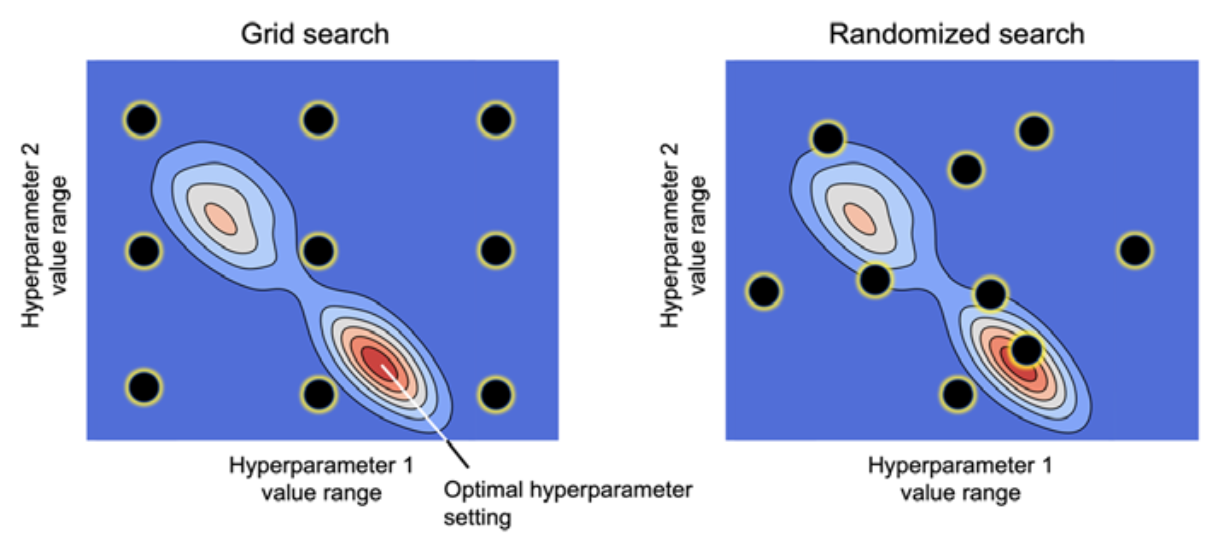
\includegraphics{figures/grid_search_vs_random_search.png}
% 	\caption{Comparison of grid search and randomized for sampling $9$ different hyperparameter configurations}
% 	\label{fig:gridsearch_vs_randomsearch}
% \end{figure}

% A third approach and the one we tried in this project is to perform a \textbf{Bayesian Search} which is basically similar to random search but modelise the hyperparameters space probabilisticly to optimize the research of the best set of hyperparameters. 

\subsection{Linear regression}

The linear regression has no hyperparameters to tune so we just ran a cross-validation for each set of features we decided to keep. The results show us that the best linear model is the one with the $\textbf{30}$ best features selected.

\begin{table}[H]
	\centering
	\begin{tabular}{ccc} \toprule
	  & \multicolumn {2}{c}{scores} \\\cmidrule(lr) {2-3}
	  \#features         & validation rmse (\$)             & test rmse (\$) \\\hline
	  $5$        		& $1.629e08$                      	& $1.154e08$ \\
	  $10$        		& $1.009e08$                        & $1.041e08$ \\
	  $15$        		& $7.850e07$                        & $9.070e07$ \\
	  $20$             	& $7.166e07$                        & $8.836e07$ \\
	  $25$             	& $6.813e07$                        & $8.738e07$ \\
	  $\textbf{30}$     & $\textbf{6.740e07}$               & $\textbf{8.539e07}$ \\
	  $35$             	& $6.649e07$                        & $8.827e07$ \\
	  $40$             	& $6.984e07$                        & $8.892e07$ \\
	  \\\hline
	\end{tabular}
	\caption{Cross-validation results of linear regression model}
	\label{tab:linear-regression-results}
\end{table}

\subsection{K-Nearest Neighbors}

For the K-Nearest Neighbors model, we need to take care of adjusting the number of neighbors hyperparameter. Indeed, a value too low will induce overfitting and a value too high will induce underfitting. Moreover, because this algorithm suffers a lot from the curse of dimensionnality, we ran it with a smaller subset of features: $[3,5,7,9,11,13,15]$. We grid searched for a number of neighbors between $1$ and $50$ first but as you can see on the figure below, this model overfits with a number of neighbors approximatively less than $7$. Then, its performance slightly decrease as this number increases.

\begin{figure}[H]
	\centering
	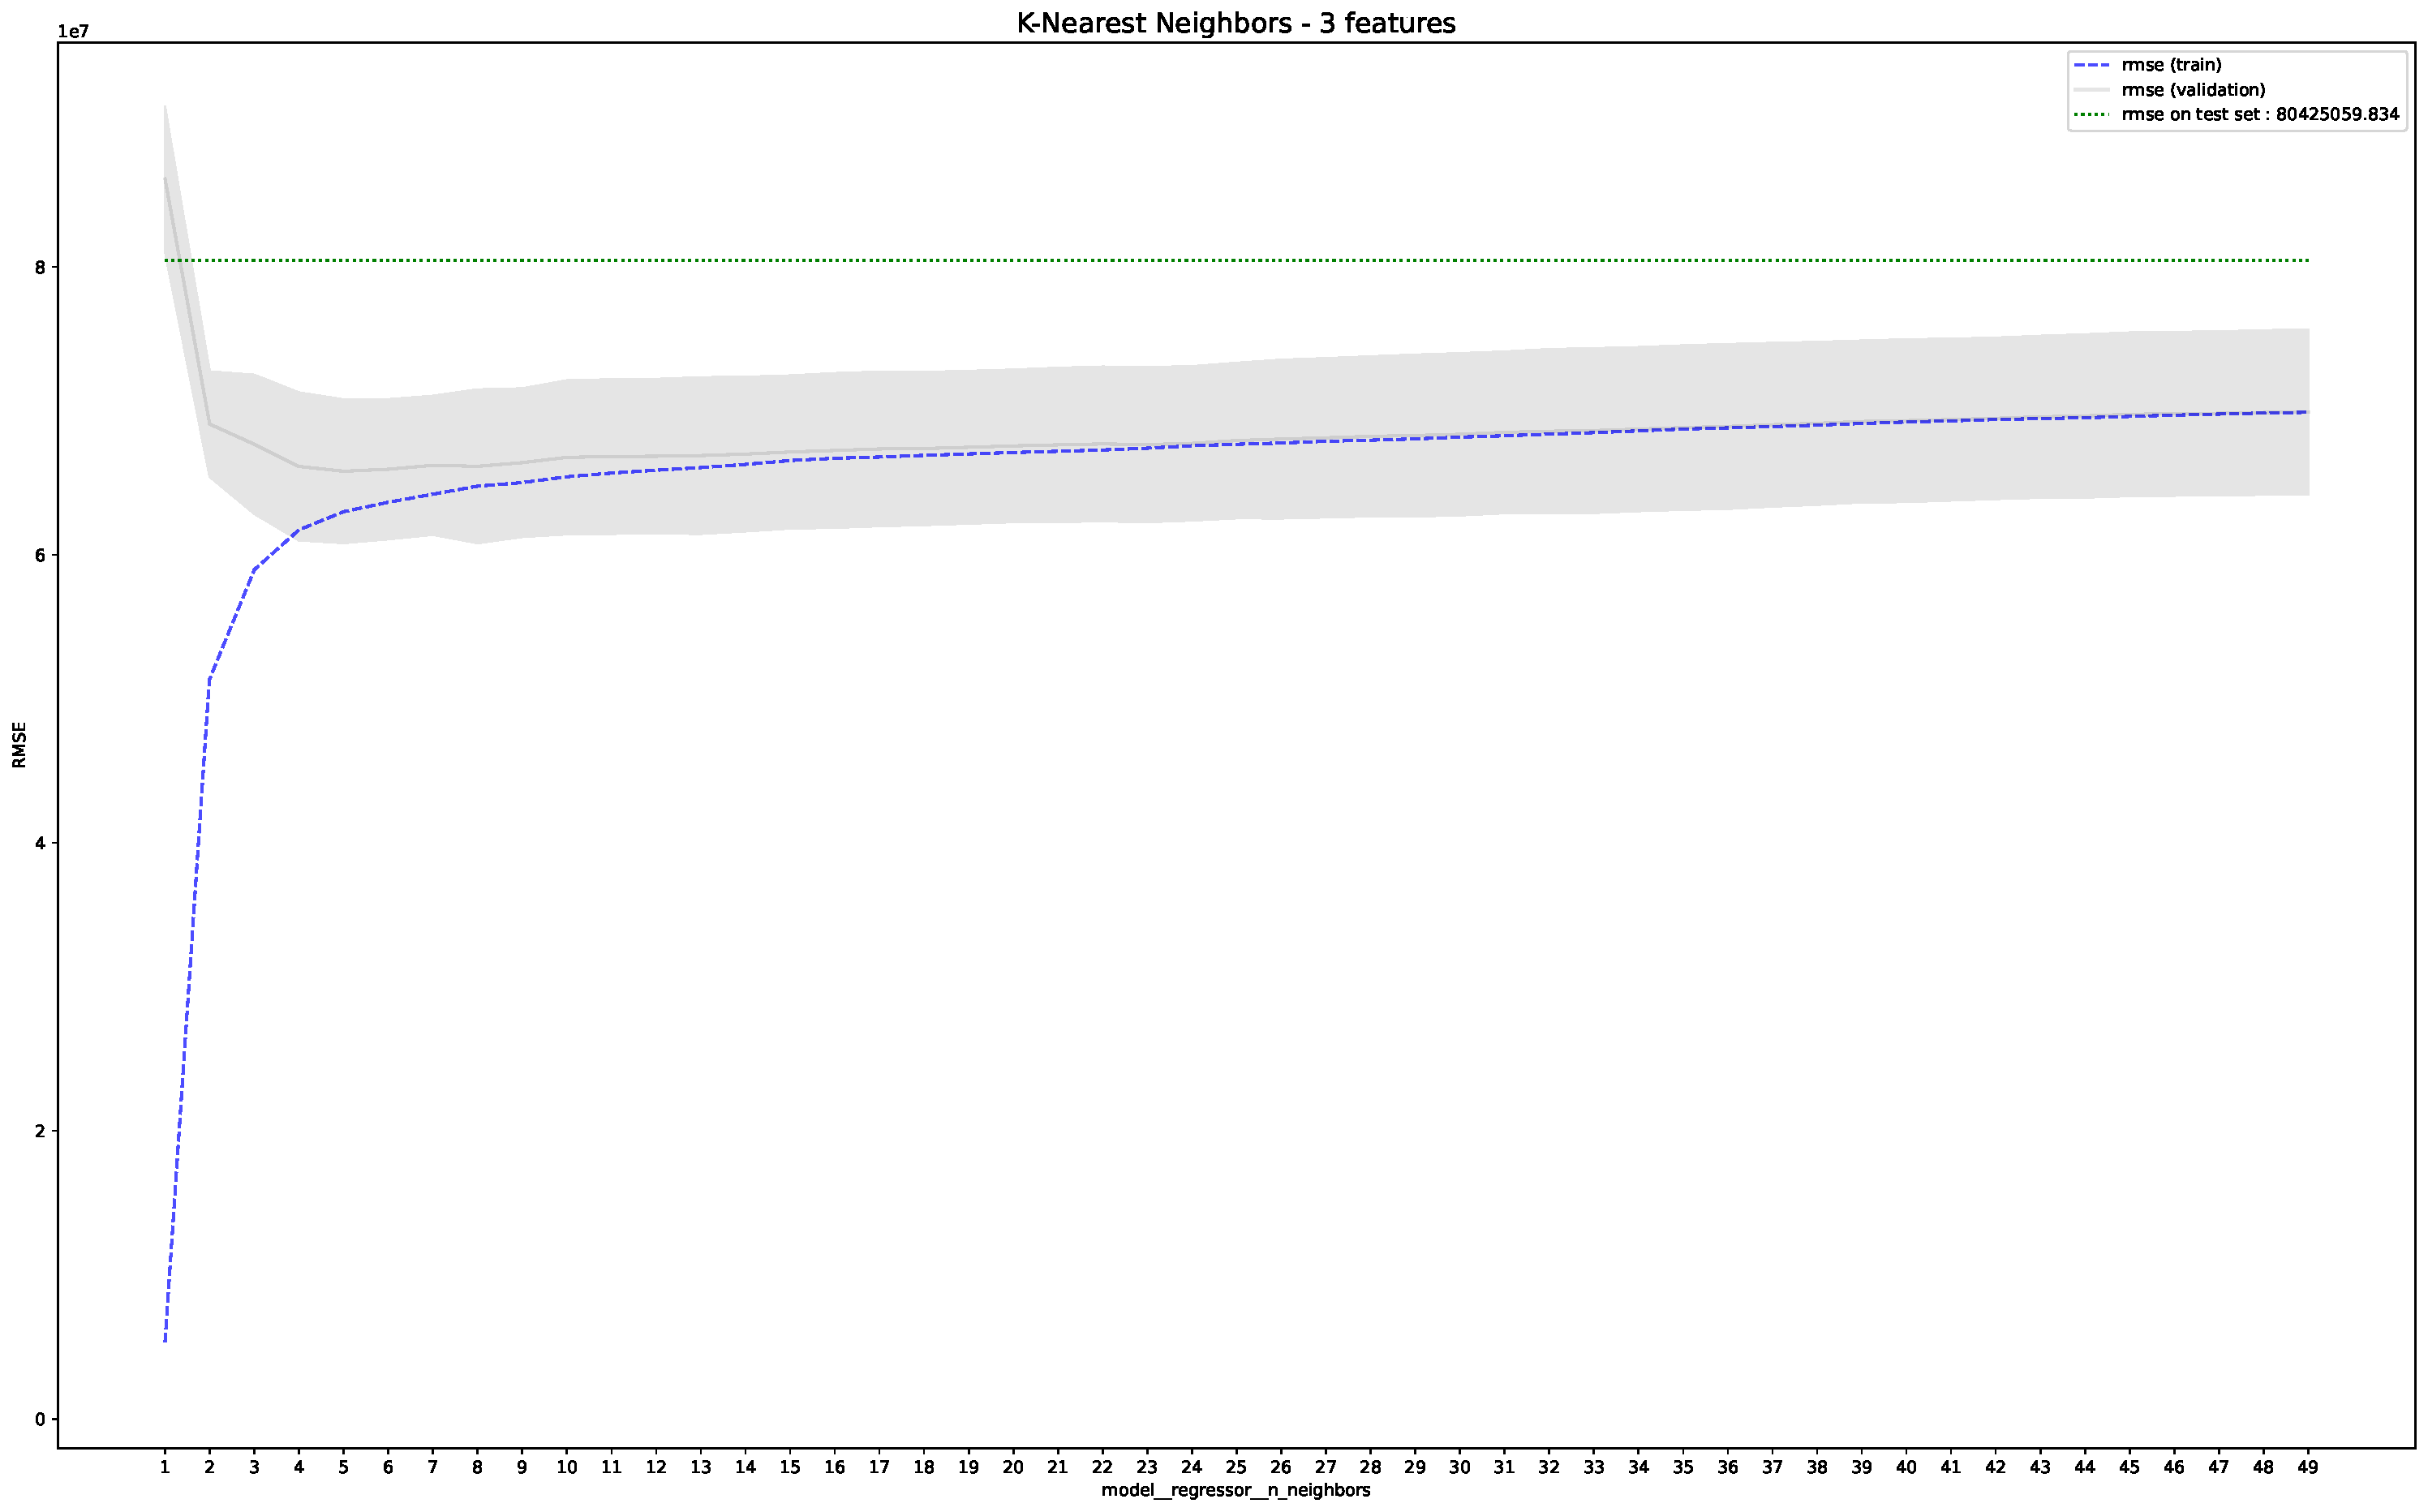
\includegraphics{figures/knn_eval.pdf}
	\caption{RMSE score with respect to the number neighbors for the best K-Nearest Neighbors model}
	\label{fig:knn_eval1}
\end{figure}

We chose to run this algorithm again but this time starting from $7$ neighbors up to $50$

\begin{figure}[H]
	\centering
	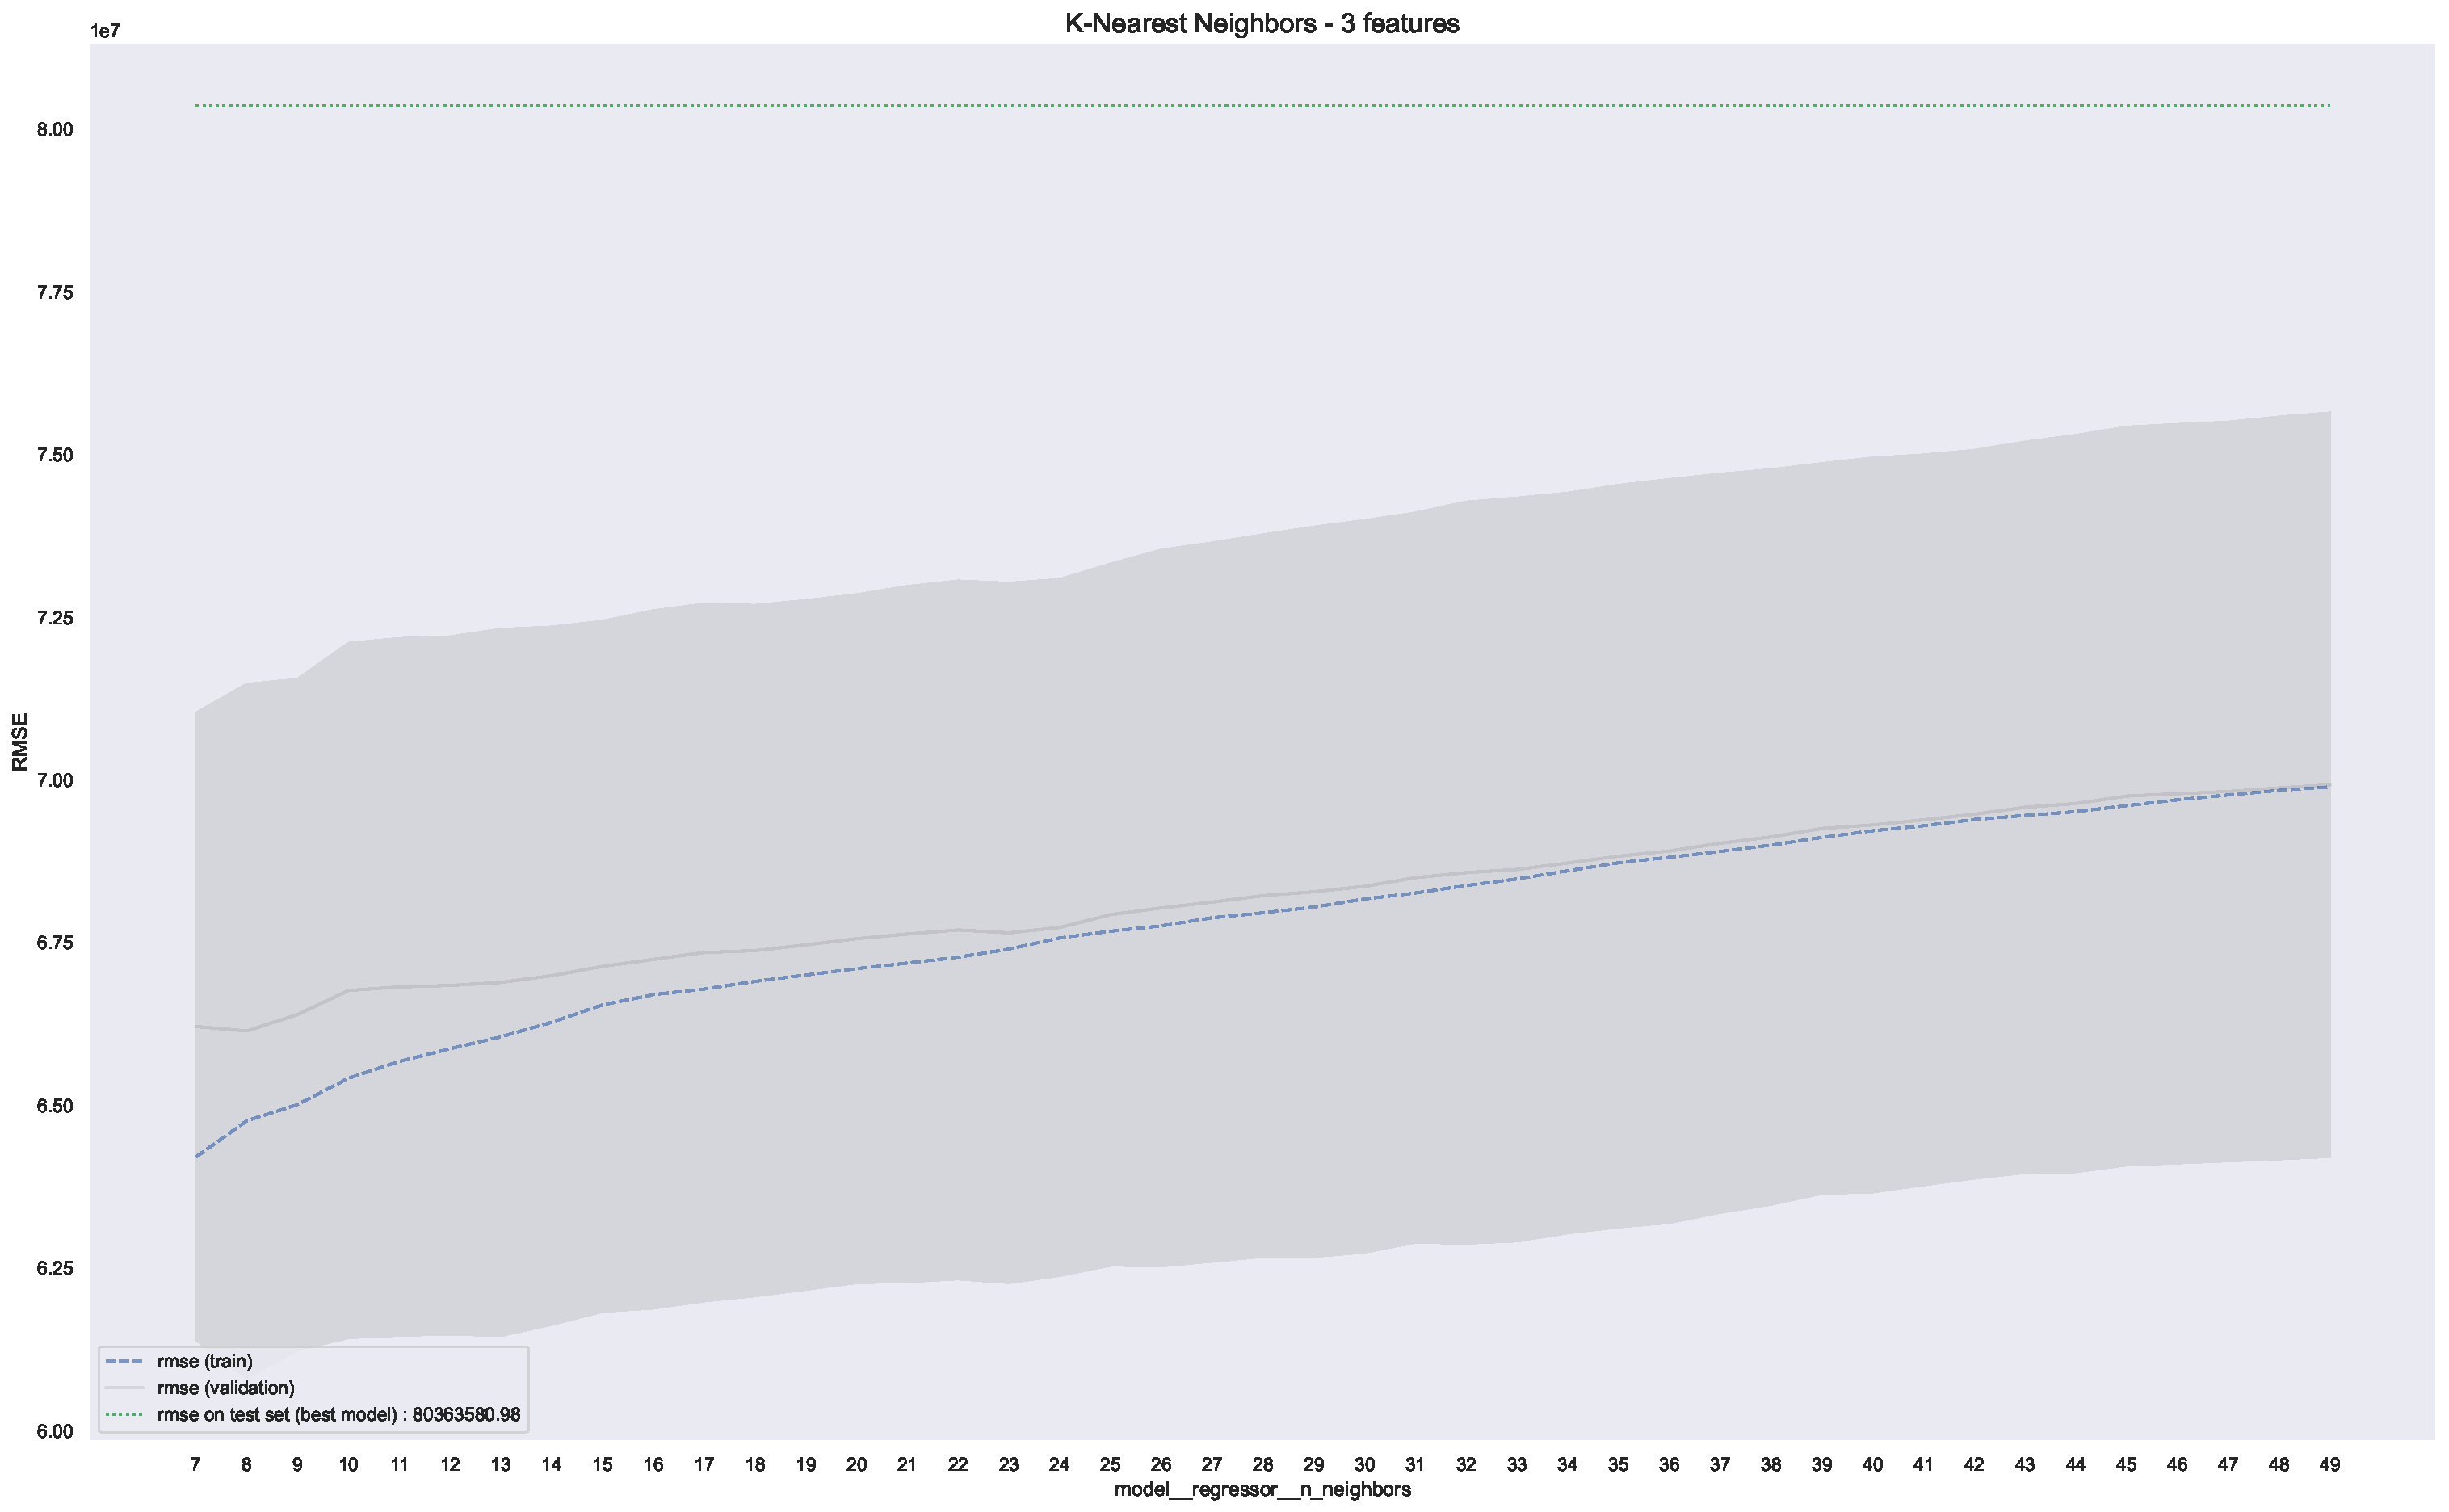
\includegraphics{figures/knn_eval2.pdf}
	\caption{RMSE score with respect to the number neighbors for the best K-Nearest Neighbors model}
	\label{fig:knn_eval2}
\end{figure}

You can see the results of this second pass on the following table,

\begin{table}[H]
	\centering
	\begin{tabular}{ccc} \toprule
	  & \multicolumn {2}{c}{scores} \\\cmidrule(lr) {2-3}
	  \#features         & validation rmse (\$)             & test rmse (\$) \\\hline
	  $\textbf{3}$        		& $\textbf{6.614e07}$                      	& $\textbf{8.036e07}$ \\
	  $5$        		& $6.642e07$                        & $8.166e07$ \\
	  $7$        		& $6.572e07$                        & $8.124e07$ \\
	  $9$             	& $6.997e07$                        & $8.481e07$ \\
	  $11$             	& $6.980e07$                        & $8.541e07$ \\
	  $13$             	& $7.691e07$                        & $9.440e07$ \\
	  $15$             	& $7.677e07$                        & $9.440e07$ \\
	  \\\hline
	\end{tabular}
	\caption{Cross-validation results of K-Nearest Neighbors model}
	\label{tab:knn-results}
\end{table}

The best model is the one with the $\textbf{3}$ best features and has $8$ neighbors.

\subsection{Multi-Layer Perceptron}

Since the multi-layer perceptron has the ability to set weights to zero, we can make the hypothesis that the feature selection will have less influence. Therefore, we wanted to test that model on a greater number of features. We also tested with all the features. We tested different number of layers and neurons per layers as well as different activation functions. We can observe that two layers gives the best results and adding more layers to the network tends to decrease the model performance.

\begin{figure}[H]
	\centering
	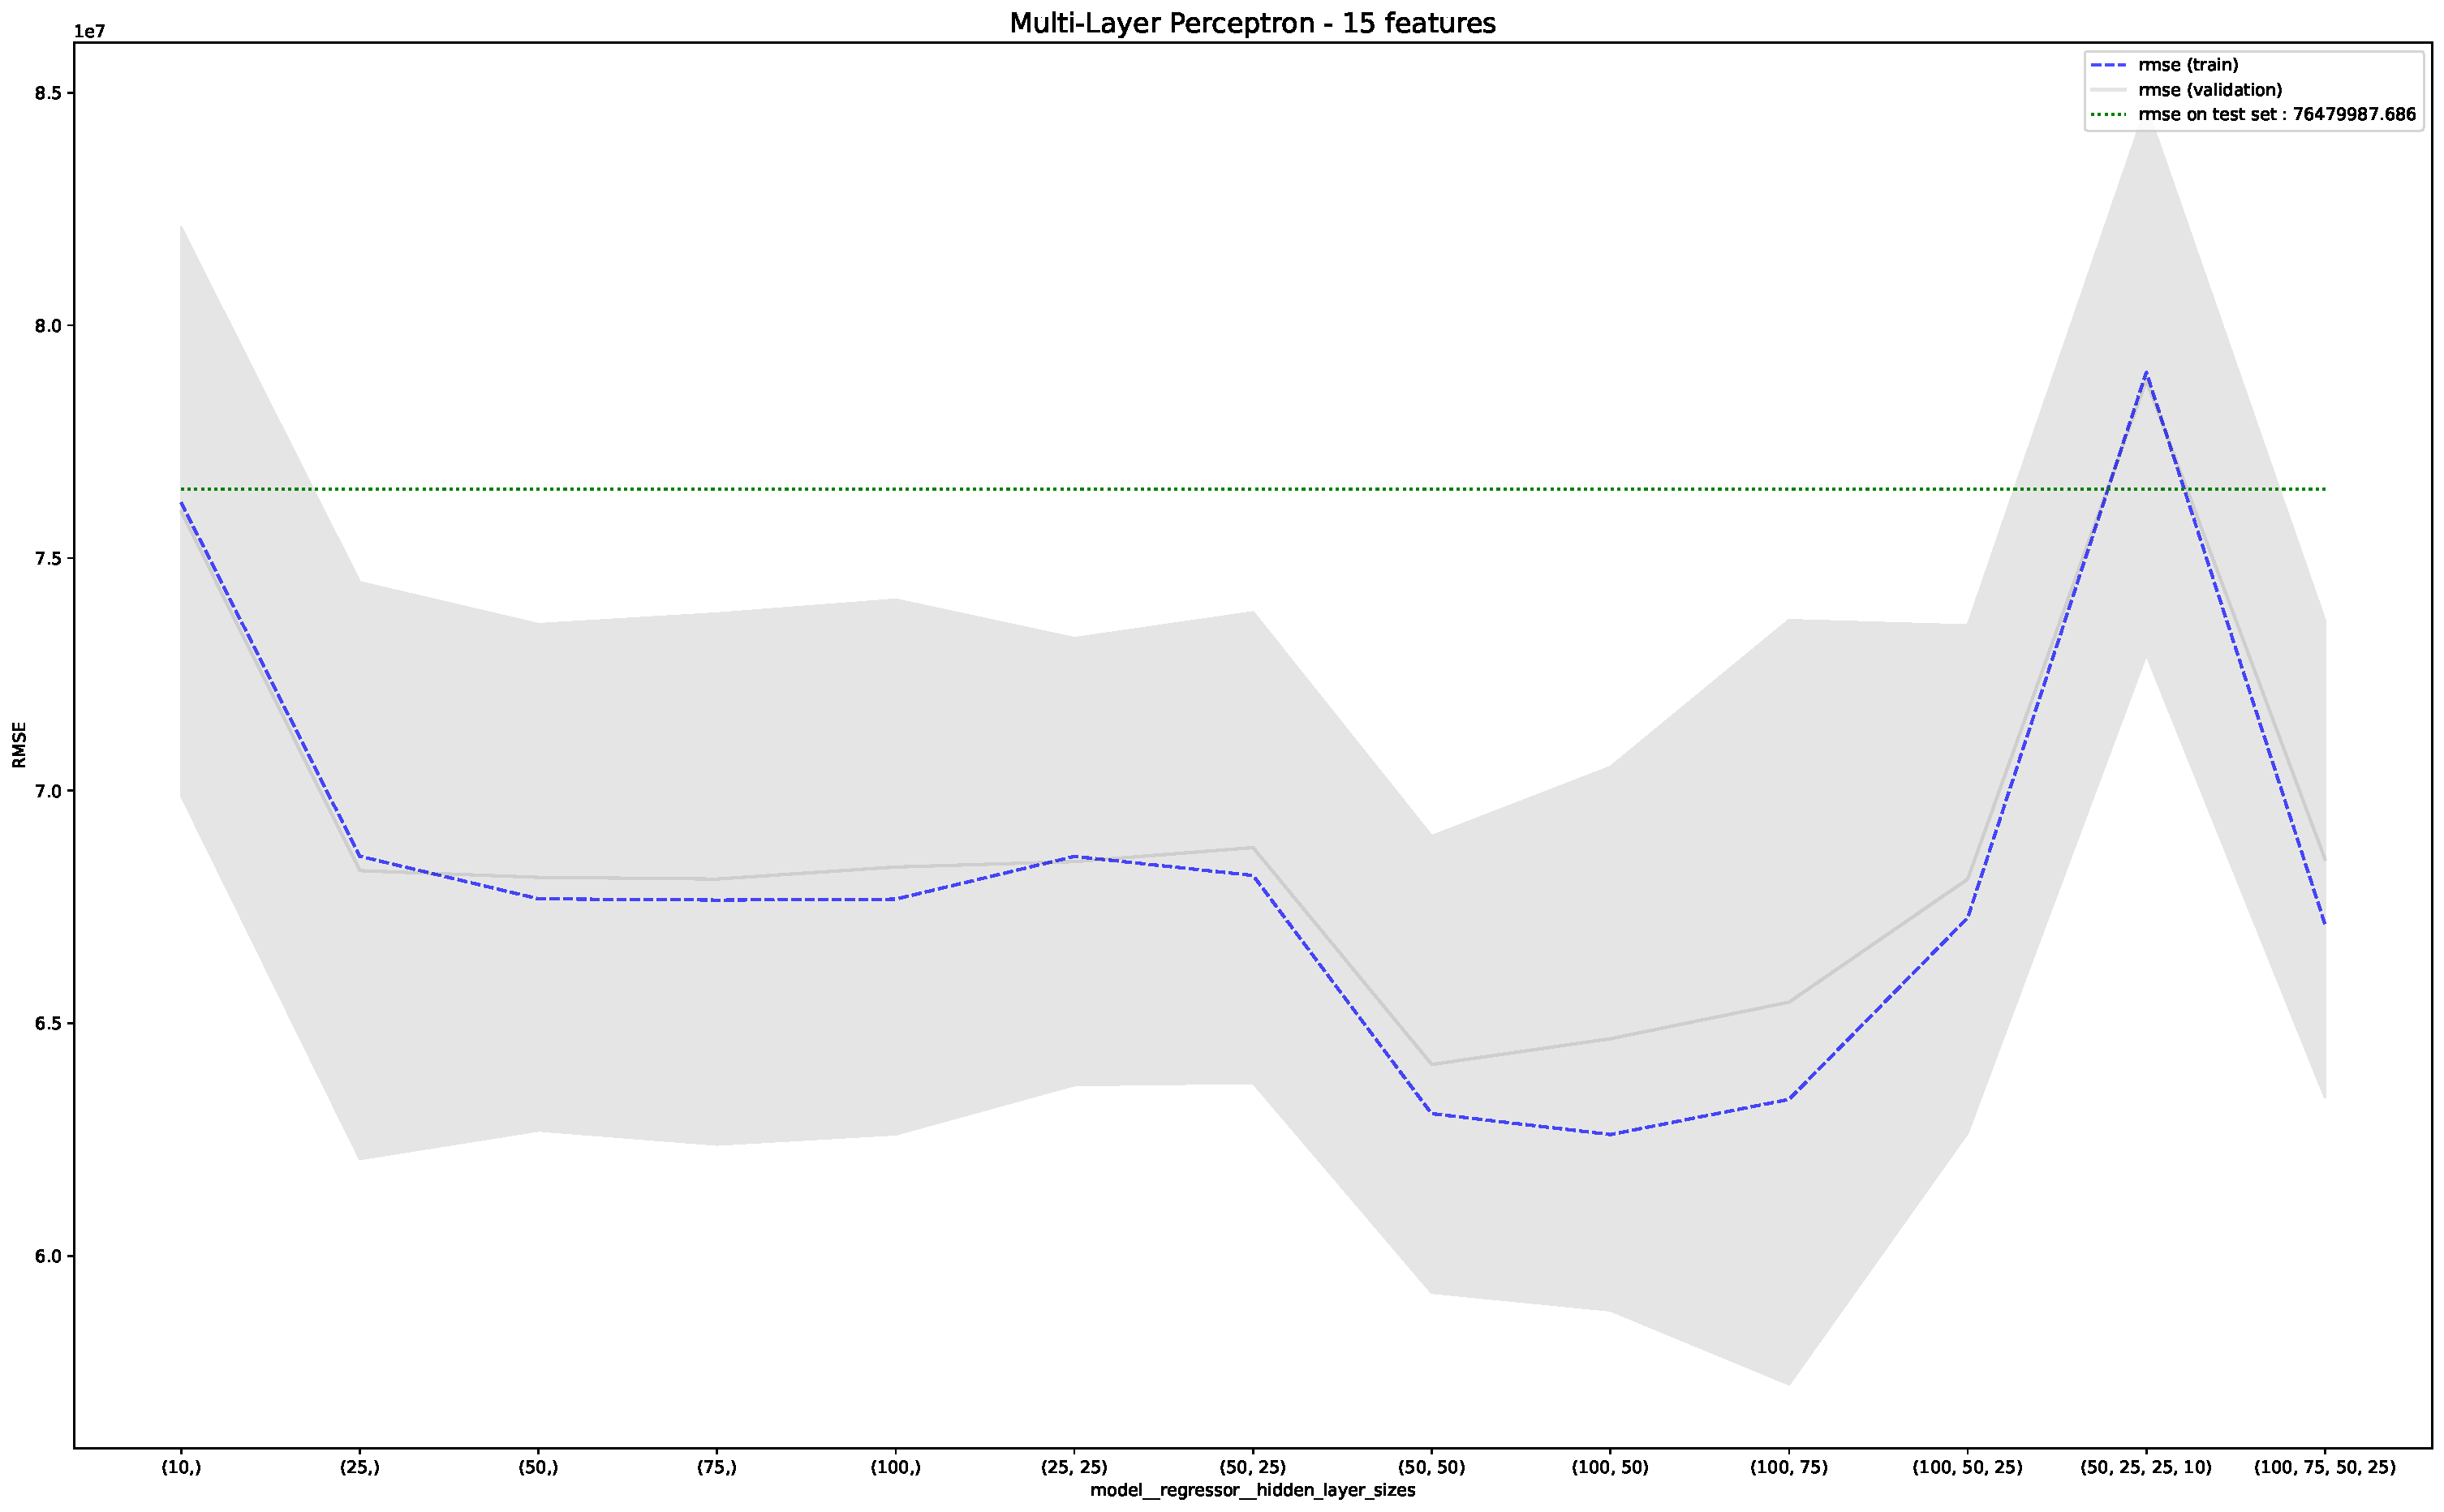
\includegraphics{figures/mlp_eval1.pdf}
	\caption{RMSE score with respect to the number of hidden layers and their sizes for the best multi-layer perceptron model}
	\label{fig:mlp_eval1}
\end{figure}

The results are summarised in the following table,
\begin{table}[H]
	\centering
	\begin{tabular}{ccc} \toprule
	  & \multicolumn {2}{c}{scores} \\\cmidrule(lr) {2-3}
	  \#features         & validation rmse (\$)             & test rmse (\$) \\\hline
	  $5$        		& $6.674e07$                      	& $8.096e07$ \\
	  $\textbf{15}$     & $\textbf{6.367e07}$               & $\textbf{7.647e07}$ \\
	  $25$        		& $6.716e07$                        & $8.272e07$ \\
	  $35$             	& $6.674e07$                        & $8.637e07$ \\
	  all             	& $6.739e07$                        & $8.289e07$ \\
	  \\\hline
	\end{tabular}
	\caption{Cross-validation results of Multi-Layer perceptron model}
	\label{tab:mlp-results}
\end{table}

The best model is the one with the $\textbf{15}$ best features and has its first layer with $100$ neurons and its second layer with $50$ neurons. It uses a $\tanh{\cdot}$ activation function and has a starting learning rate of $0.001$.

\subsection{Random Forest}

A random forest is an ensemble technique that combines multiple decision trees. As a consequence, it has a better generalization performance than a single decision tree due to randomness which decrease the model's variance. Another thing to note is that it is little sensitive to outliers and do not require much hyperparameters tuning. For this model, we performed a \textbf{Bayesian Search} with $30$ iterations. Maybe we didn't find the best model but it still should be a good model. Moreover, considering the number of hyperparameters we wanted to try, it allowed use to win much computational time. 

\begin{figure}[H]
	\centering
	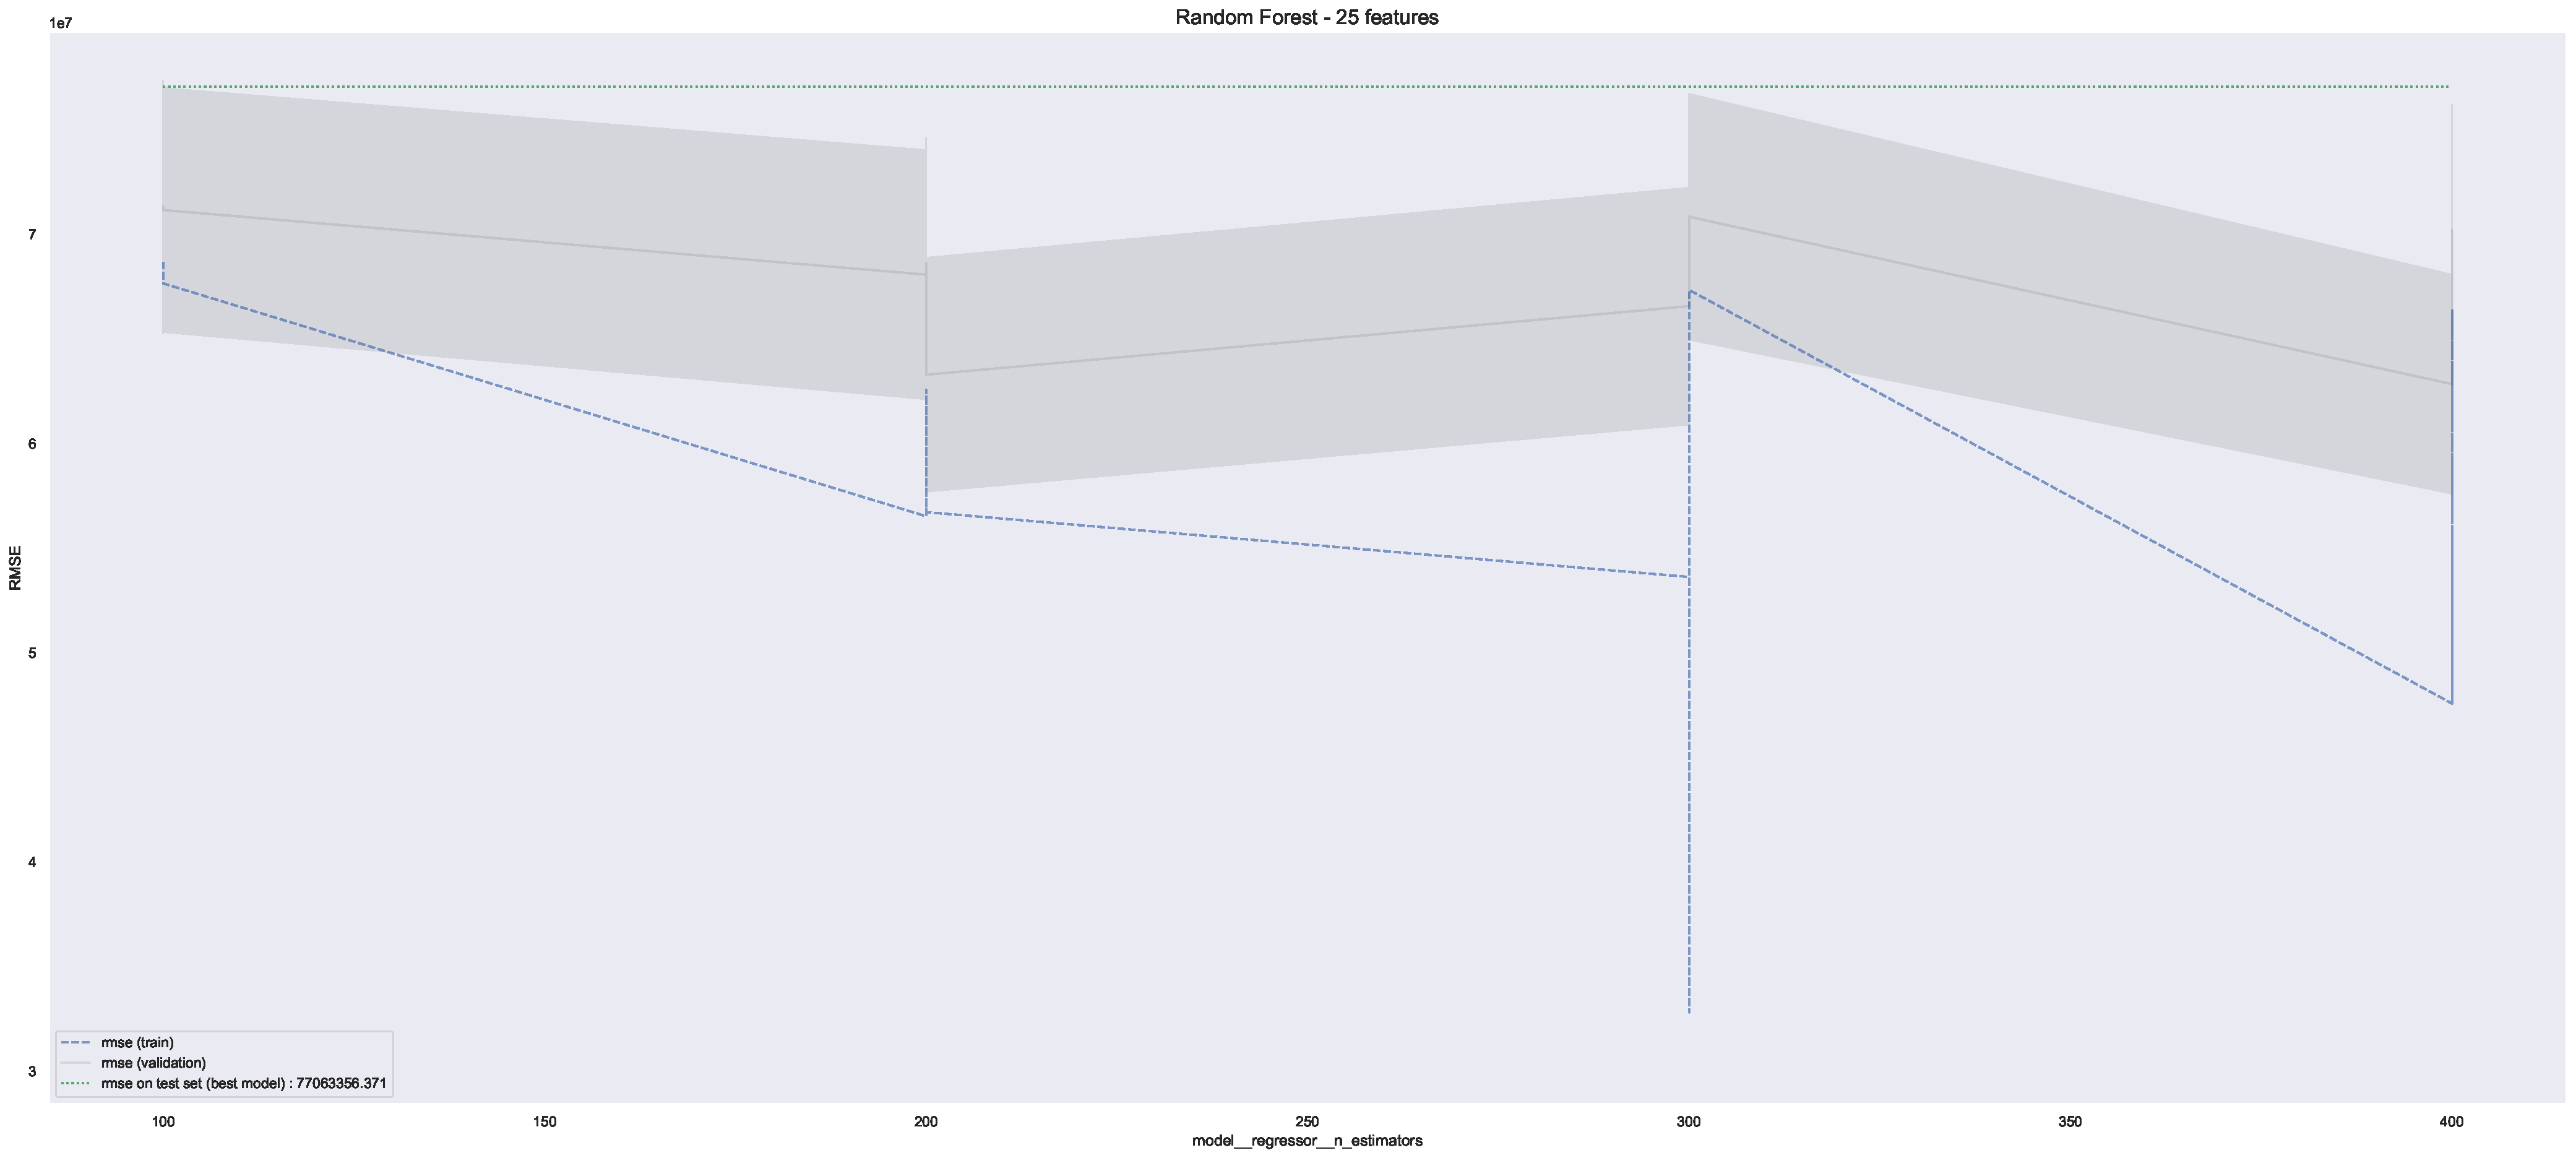
\includegraphics{figures/rf_eval.pdf}
	\caption{RMSE score with respect to the number trees for the best random forest model}
	\label{fig:rf_eval}
\end{figure}

\begin{table}[H]
	\centering
	\begin{tabular}{ccc} \toprule
	  & \multicolumn {2}{c}{scores} \\\cmidrule(lr) {2-3}
	  \#features         & validation rmse (\$)             & test rmse (\$) \\\hline
	  $5$        		& $6.390e07	$                      	& $8.131e07$ \\
	  $10$        		& $6.333e07$                        & $7.785e07$ \\
	  $15$        		& $6.267e07$                        & $7.816e07$ \\
	  $\textbf{20}$             	& $\textbf{6.316e07}$                        & $\textbf{7.741e07}$ \\
	  $25$             	& $6.271e07$                        & $7.774e07$ \\
	  \\\hline
	\end{tabular}
	\caption{Cross-validation results of Random Forest model}
	\label{tab:rf-results}
\end{table}

The best model is the one with the $\textbf{20}$ best features. It uses $200$ estimators.